\begin{activity}\label{A:0.4.1}

Without using a calculator or computer, match the functions $e^{x}$, $\ln{x}$, $x^{2}$, and $x^{1/2}$ to their graphs:

% \begin{figure}[ht!]     
	\begin{center}         
		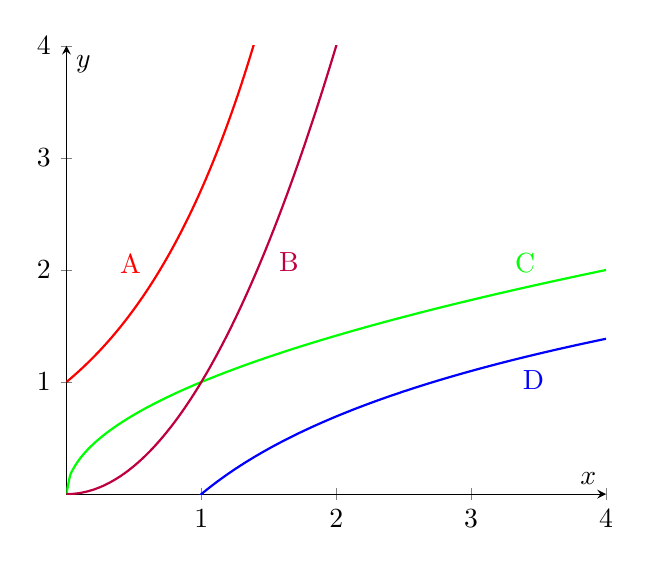
\begin{tikzpicture}[scale=1]             
			\begin{axis}[axis lines=center, xlabel={$x$}, ylabel={$y$}, domain=0:4,
							ymin=0, ymax=4,xmin=0,xmax=4]
				\addplot[smooth, thick, blue, samples=150] {ln(x)}
						[below right] node[pos=0.9] {\color{blue} D};
				\addplot[smooth, thick, red, samples=150] {exp(x)}
						[above left] node[pos=0.02] {\color{red} A};
				\addplot[smooth, thick, green, samples=150] {x^(1/2)}
						[above left] node[pos=0.9] {\color{green} C};
				\addplot[smooth, thick, purple, samples=150] {x^(2)}
						[below right] node[pos=0.168] {\color{purple} B};
			\end{axis}
		\end{tikzpicture}     
	\end{center}     
% \caption{}     
% \label{F:0.4.Act1} 
% \end{figure}

Without using a calculator or computer, match the functions $\log_{2}{x}$, $\log_{4}{x}$, $\log_{5}{x}$, and $\log_{10}{x}$ to their graphs:

% \begin{figure}[ht!]     
	\begin{center}
    		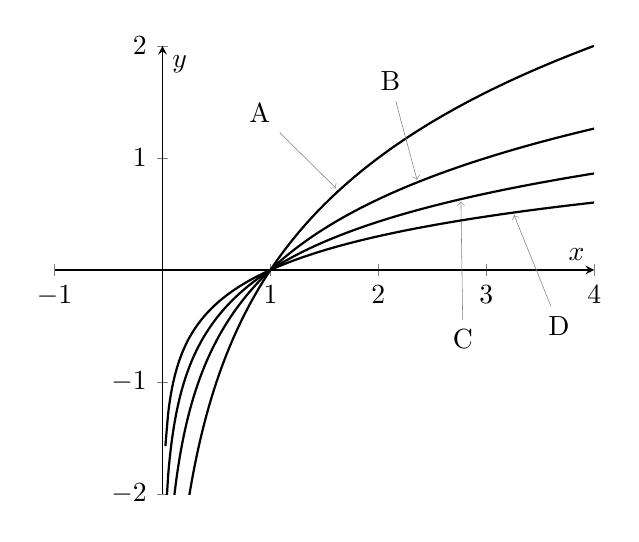
\begin{tikzpicture}[scale=1]
			\begin{axis}[axis lines=center, xlabel={$x$}, ylabel={$y$}, domain=0:4,
							ymin=-2,ymax=2,xmin=-1,xmax=4]
				\addplot[smooth, thick, black, samples=150] {ln(x)/ln(2)}
						node[pos=0.7, pin={[pin distance=1cm, pin edge={<-}]135:A}, inner sep=0pt]{};
				\addplot[smooth, thick, black, samples=150] {ln(x)/ln(3))}
						node[pos=0.75, pin={[pin distance=1cm, pin edge={<-}]95:B}, inner sep=0pt]{};
				\addplot[smooth, thick, black, samples=150] {ln(x)/ln(5)}
						node[pos=0.78, pin={[pin distance=15mm, pin edge={<-}]271:C}, inner sep=0pt]{};
				\addplot[smooth, thick, black, samples=150] {ln(x)/ln(10)}
						node[pos=0.85, pin={[pin distance=12mm, pin edge={<-}]285:D}, inner sep=0pt]{};
			\end{axis}
		\end{tikzpicture}
	\end{center} 
% \caption{}     
% \label{F:0.4.Act2} 
% \end{figure}

\end{activity}\aftera
